\documentclass{../tools/letask}
\usepackage{../tools/iunits}
\setlist{resume, leftmargin=1cm, topsep=0cm, resume}

\newcommand{\LabTitle}{Дифракция света\\[0.1cm]на ультразвуковой волне в жидкости}

\begin{document}
\begin{titlepage}
\center % Center everything on the page
 
%----------------------------------------------------------------------------------------
%	HEADING SECTIONS
%----------------------------------------------------------------------------------------

\textsc{\LARGE Московский\\[-0.2cm]Физико-Технический Институт\\[0.1cm]\large (государственный университет)}\\[1.5cm] % Name of your university/college
\textsc{\Large Кафедра общей физики}\\[0.1cm] % Major heading such as course name
\textsc{\large Лабораторная работа, 4 семестр}\\[0.5cm] % Minor heading such as course title

%----------------------------------------------------------------------------------------
%	TITLE SECTION
%----------------------------------------------------------------------------------------

\HRule
\\[0.8cm]
{ \huge \bfseries \LabTitle}
\\[0.8cm] % Title of your document
\HRule
\\[1.5cm]


 
%----------------------------------------------------------------------------------------
%	AUTHOR SECTION
%----------------------------------------------------------------------------------------

\begin{minipage}{0.4\textwidth}
	\begin{flushleft} \large
		\textsf{Студент}
		
		Георгий \textsc{Корепанов} \\[-0.15cm]
		512 группа
	\end{flushleft}
\end{minipage}
~
\begin{minipage}{0.4\textwidth}
	\begin{flushright} \large
		\textsf{Преподаватель}
		
		Сергей Львович\\[-0.15cm]
		\textsc{Клёнов} % Supervisor's Name
	\end{flushright}
\end{minipage}

\begin{bottompar}
	\begin{center}
		
\includegraphics[width = 80 mm]{../tools/img/logo.jpg}
	\end{center}
	{\large \today}

\end{bottompar}
\vfill % Fill the rest of the page with whitespace

\end{titlepage}


\section{Цель работы}
\begin{enumerate}
\item
Изучение дифракции света на \textsf{фазовой решётке}, сформированной акустической волной:
\begin{enumerate}
\item Наблюдение дифракции Фраунгофера
\item Наблюдение методом тёмного поля
\end{enumerate}

\end{enumerate}
\section{Основная теория}
\subsection{Параметры акустического транспаранта}
Распределение показателя преломления:
$$n=n_0(1+m\cos \Omega x).$$
Фазовое распределение на задней поверхности:
$$\varphi = knL = \varphi_0(1+m\cos \Omega x).$$

Условие тонкого транспаранта:
$$m \ll \dfrac{\Lambda}{L} \sqrt{\dfrac{\lambda}{L}},$$
где 
\begin{align*}
&\Lambda \text{ -- длина УЗ волны,}\\
&\lambda \text{ -- длина световой волны,}\\
&\Omega \text{ -- волновое число УЗ волны,}\\
&L \text{ -- толщина слоя жидкости в кювете.}
\end{align*}

\subsection{Фурье-спектр фазово модулированной волны}
Световое поле состоит из плоских волн, распространяющихся под углами 
$$\Lambda \sin \theta_m = m \lambda, \quad m \in \mathbb{Z}.$$

\subsection{Определение скорости рапространения ультразвуковых волн}
Определяя углы $\theta_m$ по расстоянию между дифракционными полосами $l_m$
$$l_m = mf\dfrac{\lambda}{\Lambda},$$
определим длину УЗ волны $\Lambda$.
При измерениях методом тёмного поля $\Lambda$ измеряется непосредственно как удвоенное расстояние между тёмными полосами.
Скорость УЗ волны $\upsilon$ может быть вычислена, таким образом, при известной частоте генератора:
$$\upsilon= \Lambda \nu.$$

\section{Схемы установки}
\subsection{Дифракция на фазовой решётке}
\begin{figure}[H]
\centering
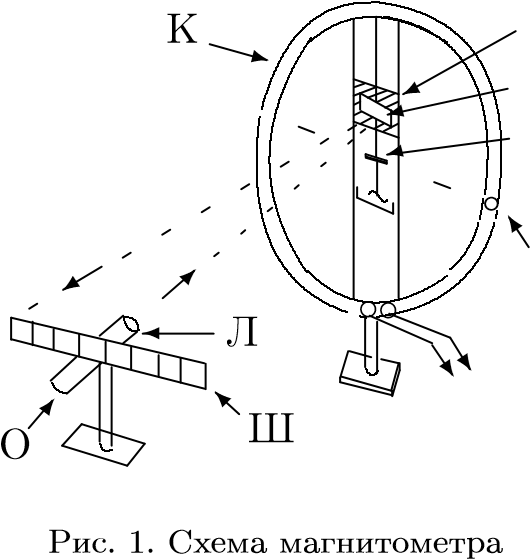
\includegraphics[width =\textwidth]{1}
\caption{Схема первой установки}
\end{figure}
\subsection{Метод тёмного поля}
\begin{figure}[H]
\centering
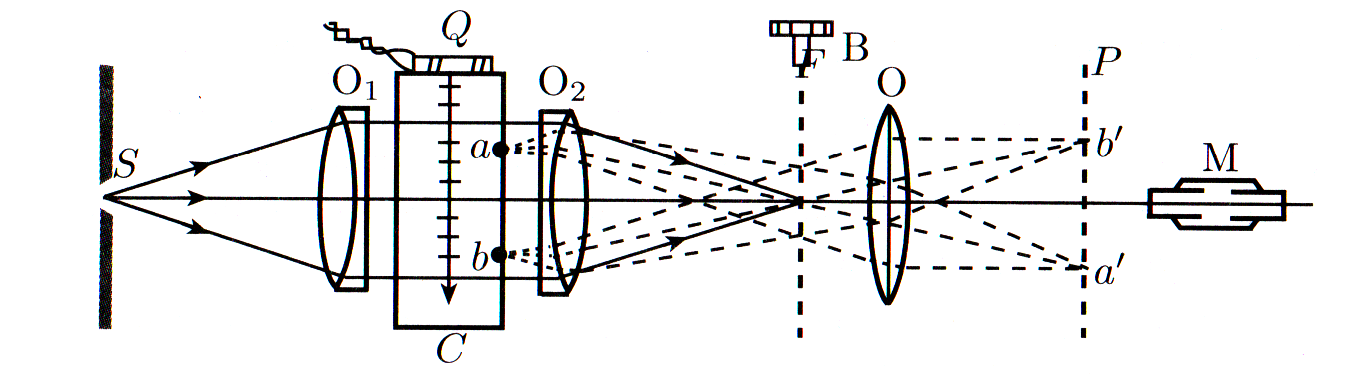
\includegraphics[width =\textwidth]{2}
\caption{Схема второй установки}
\end{figure}

\end{document}